\documentclass[a4paper,10pt]{IEEEtran}
%\usepackage{scrpage2}
\usepackage[latin1]{inputenc}
\usepackage[pdftex,colorlinks,linkcolor=black,citecolor=black]{hyperref}
\usepackage{amsmath}
\usepackage{amssymb}
\usepackage{amsthm}
\usepackage{latexsym} 
\usepackage{bbm}
\usepackage{tikz}
\usepackage{flushend}
\usetikzlibrary{shapes}
%\usetikzlibrary{snakes}
%\usepackage{pgflibraryshapes}
%\usepackage{pgflibrarysnakes}
\usepackage{xspace}
\usepackage{rotating}
\usepackage{mathrsfs}


\newtheorem{lem}{Lemma}
\newtheorem{theo}[lem]{Theorem}
\newtheorem{defi}[lem]{Definition}
\newtheorem{corol}[lem]{Corollary}

\newcommand{\LL}{\mathcal{L}}
\newcommand{\NN}{\mathbbm{N}}
\newcommand{\ZZ}{\mathbbm{Z}}
\newcommand{\AP}{\mathit{AP}}
\newcommand{\SyntComp}{\textsc{SyntComp}}
\newcommand{\FALSE}{\mathbf{false}}
\newcommand{\TRUE}{\mathbf{true}}
\newcommand{\BB}{\mathbbm{B}}
\newcommand{\SpaceforresultsA}{$\quad$\\$\quad$\\$\quad$\\$\quad$\\$\quad$\\}
\newcommand{\SpaceforresultsB}{\SpaceforresultsA\SpaceforresultsA}
\newcommand{\SpaceforresultsC}{\SpaceforresultsB\SpaceforresultsB}
\newcommand{\SpaceforresultsD}{\SpaceforresultsC\SpaceforresultsC}
\newcommand{\Spaceforresults}{\SpaceforresultsD\SpaceforresultsD}
\newcommand{\newterm}{\textit}
%\newcommand{\existsinfmany}{\mathop{\exists}\limits_{\infty}}
\newcommand{\existsinfmany}{\mathop{\exists}^{\infty}}
\newcommand{\true}{\TRUE}
\newcommand{\false}{\FALSE}
\hyphenation{rea-li-sa-bi-li-ty ge-ne-ra-lised li-mi-ted}
\allowdisplaybreaks

\author{\IEEEauthorblockN{R\"udiger Ehlers \\}
\IEEEauthorblockA{University of Bremen \& DFKI GmbH\\
Germany
}}

%\cfoot[]{Blubb}
%\pagestyle{scrplain}
\begin{document}
%\pagestyle{scrplain}
\title{Simple Factory Assembly Line Benchmarks}
\maketitle

\section{Basic Setup}
%
\noindent This benchmark set is concerned with a very simple assembly line. Figure \ref{fig:assemblyLineDrawing} depicts the scenario graphically. We have a conveyor belt with $n=7$ places that are reachable by two manipulator arms, and on each of the places, there is an object. Before an object is pushed off the belt, $m=4$ tasks have to be performed on the object. Every $k$ cycles, the belt rotates by one place and delivers a new object. At every step, a manipulator arm can perform one task on the object underneath it. The manipulator arms can also move by one place, but they can never be at the same place and can also not overtake each other. The objects come with one task already having been performed on them. Initially, the belt is filled with objects for which all tasks have been performed already.


The scenarios in this benchmark set have many input and output signals, but only few counters. Thus, they aim at complementing counter-rich other benchmarks in the \SyntComp.

\subsection{Input and output signals}
%
\noindent We have the following signals:
\begin{itemize}
\item Boolean inputs to the system to be synthesized:
\begin{enumerate}
\item signals $\mathit{ck}_0, \ldots, \mathit{ck}_{|\mathit{ck}|}$ that encode the binary representation of a counter for how many steps are left until $k$ steps without belt motion have been witnessed
\item signals $\{\mathit{p}_{i,j} \}_{0 \leq i < n, 0 \leq j < m}$ that encode whether task $j$ has already been performed on the object at position $i$ 
\end{enumerate}
\item Boolean outputs of the system to be synthesized:
\begin{enumerate}
\item signals $\mathit{arm1pos}_1,  \ldots, \mathit{arm1pos}_{\lceil \log_2 n \rceil}$ to encode the position of the first arm
\item signals $\mathit{arm2pos}_1,  \ldots, \mathit{arm2pos}_{\lceil \log_2 n \rceil}$ to encode the position of the second arm
\item signals $\mathit{arm1action}_1,  \ldots, \mathit{arm1action}_{\lceil \log_2 m \rceil}$ to encode which task the first arm is currently performing
\item signals $\mathit{arm2action}_2,  \ldots, \mathit{arm1action}_{\lceil \log_2 m \rceil}$ to encode which task the first arm is currently performing
\end{enumerate}
\end{itemize}



\begin{figure}[t]
\centering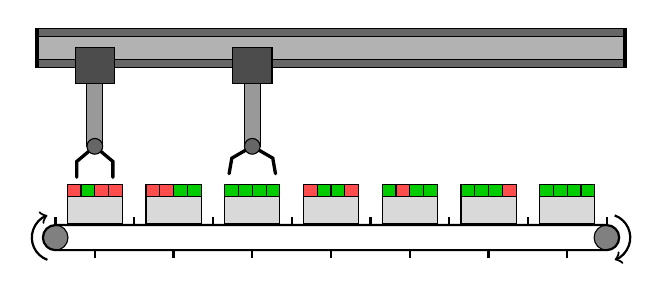
\begin{tikzpicture}
\draw[fill=black!50!white] (0,-1/2/pi) circle (1/2/pi);
\draw[fill=black!50!white] (7,-1/2/pi) circle (1/2/pi);
\draw[thick] (0,0.0) -- (7,0.0) arc (90:-90:1/2/pi) -- +(-7,0) arc (-90:-270:1/2/pi) -- cycle;

\draw[color=black,thick] (0,0.0) -- +(0,0.1cm);
\draw[color=black,thick] (1,0.0) -- +(0,0.1cm);
\draw[color=black,thick] (2,0.0) -- +(0,0.1cm);
\draw[color=black,thick] (3,0.0) -- +(0,0.1cm);
\draw[color=black,thick] (4,0.0) -- +(0,0.1cm);
\draw[color=black,thick] (5,0.0) -- +(0,0.1cm);
\draw[color=black,thick] (6,0.0) -- +(0,0.1cm);
\draw[color=black,thick] (7,0.0) -- +(0,0.1cm);
\draw[color=black,thick] (0.5,-1/pi) -- +(0,-0.1cm);
\draw[color=black,thick] (1.5,-1/pi) -- +(0,-0.1cm);
\draw[color=black,thick] (2.5,-1/pi) -- +(0,-0.1cm);
\draw[color=black,thick] (3.5,-1/pi) -- +(0,-0.1cm);
\draw[color=black,thick] (4.5,-1/pi) -- +(0,-0.1cm);
\draw[color=black,thick] (5.5,-1/pi) -- +(0,-0.1cm);
\draw[color=black,thick] (6.5,-1/pi) -- +(0,-0.1cm);

\draw[thick,->] (0,-1/2/pi) ++(250:0.3cm) arc(250:110:0.3cm);
\draw[thick,->] (7,-1/2/pi) ++(70:0.3cm) arc(70:-70:0.3cm);

\foreach \base in {0,1,2,3,4,5,6}{

\draw[fill=black!15!white] (\base+0.15,0.015) rectangle +(0.7,0.5);
}

% Explicitly completed tasks
\draw[fill=red!70!white] (0+0.15+0*0.175,0.515) rectangle +(0.175,-0.15);
\draw[fill=green!80!black] (0+0.15+1*0.175,0.515) rectangle +(0.175,-0.15);
\draw[fill=red!70!white] (0+0.15+2*0.175,0.515) rectangle +(0.175,-0.15);
\draw[fill=red!70!white] (0+0.15+3*0.175,0.515) rectangle +(0.175,-0.15);
\draw[fill=red!70!white] (1+0.15+0*0.175,0.515) rectangle +(0.175,-0.15);
\draw[fill=red!70!white] (1+0.15+1*0.175,0.515) rectangle +(0.175,-0.15);
\draw[fill=green!80!black] (1+0.15+2*0.175,0.515) rectangle +(0.175,-0.15);
\draw[fill=green!80!black] (1+0.15+3*0.175,0.515) rectangle +(0.175,-0.15);
\draw[fill=green!80!black] (2+0.15+0*0.175,0.515) rectangle +(0.175,-0.15);
\draw[fill=green!80!black] (2+0.15+1*0.175,0.515) rectangle +(0.175,-0.15);
\draw[fill=green!80!black] (2+0.15+2*0.175,0.515) rectangle +(0.175,-0.15);
\draw[fill=green!80!black] (2+0.15+3*0.175,0.515) rectangle +(0.175,-0.15);
\draw[fill=red!70!white] (3+0.15+0*0.175,0.515) rectangle +(0.175,-0.15);
\draw[fill=green!80!black] (3+0.15+1*0.175,0.515) rectangle +(0.175,-0.15);
\draw[fill=green!80!black] (3+0.15+2*0.175,0.515) rectangle +(0.175,-0.15);
\draw[fill=red!70!white] (3+0.15+3*0.175,0.515) rectangle +(0.175,-0.15);
\draw[fill=green!80!black] (4+0.15+0*0.175,0.515) rectangle +(0.175,-0.15);
\draw[fill=red!70!white] (4+0.15+1*0.175,0.515) rectangle +(0.175,-0.15);
\draw[fill=green!80!black] (4+0.15+2*0.175,0.515) rectangle +(0.175,-0.15);
\draw[fill=green!80!black] (4+0.15+3*0.175,0.515) rectangle +(0.175,-0.15);
\draw[fill=green!80!black] (5+0.15+0*0.175,0.515) rectangle +(0.175,-0.15);
\draw[fill=green!80!black] (5+0.15+1*0.175,0.515) rectangle +(0.175,-0.15);
\draw[fill=green!80!black] (5+0.15+2*0.175,0.515) rectangle +(0.175,-0.15);
\draw[fill=red!70!white] (5+0.15+3*0.175,0.515) rectangle +(0.175,-0.15);
\draw[fill=green!80!black] (6+0.15+0*0.175,0.515) rectangle +(0.175,-0.15);
\draw[fill=green!80!black] (6+0.15+1*0.175,0.515) rectangle +(0.175,-0.15);
\draw[fill=green!80!black] (6+0.15+2*0.175,0.515) rectangle +(0.175,-0.15);
\draw[fill=green!80!black] (6+0.15+3*0.175,0.515) rectangle +(0.175,-0.15);

% Robot Arm Basis
\draw[fill=black!30!white] (-0.25,2) rectangle (7.25,2.5);
\draw[thin,fill=black!60!white] (-0.25,2) rectangle (7.25,2.1);
\draw[thin,fill=black!60!white] (-0.25,2.4) rectangle (7.25,2.5);
\draw[fill=black] (-0.25,2.0) rectangle (-0.22,2.5);
\draw[fill=black] (7.25,2.0) rectangle (7.22,2.5);

% Robot Arm 1
\draw[fill=black!40!white] (0.4,2.2) rectangle (0.6,1.0);
\draw[very thick,line cap=round] (0.5,1.0) -- ++(220:0.3cm) -- +(-90:0.2cm);
\draw[very thick,line cap=round] (0.5,1.0) -- ++(320:0.3cm) -- +(-90:0.2cm);
\draw[fill=black!60!white] (0.5,1.0) circle (0.1cm);
\draw[fill=black!70!white] (0.25,1.8) rectangle (0.75,2.25);

% Robot Arm 2
\draw[fill=black!40!white] (2.4,2.2) rectangle (2.6,1.0);
\draw[very thick,line cap=round] (2.5,1.0) -- ++(210:0.3cm) -- +(-100:0.2cm);
\draw[very thick,line cap=round] (2.5,1.0) -- ++(330:0.3cm) -- +(-80:0.2cm);
\draw[fill=black!60!white] (2.5,1.0) circle (0.1cm);
\draw[fill=black!70!white] (2.25,1.8) rectangle (2.75,2.25);

\end{tikzpicture}
\caption{Schematic drawing of a simple assembly line}
\label{fig:assemblyLineDrawing}
\end{figure}

\subsection{Specification}
\noindent The specification consists of \emph{assumptions} and \emph{guarantees}, which are connected by a \emph{strong implication} as common in GR(1) synthesis, i.e., it is the aim of the system to make sure that no guarantee is violated before some assumption is violated (see, e.g., \cite{DBLP:journals/jcss/BloemJPPS12}, section 3.3). If some assumption and some guarantee are violated in the same step, the system also satisfies its overall specification.
\begin{itemize}
\item Assumptions:
\begin{enumerate}
\item The $\mathit{ck}$ counter cycles through the values $0, \ldots, k-1$.
\item Whenever the $\mathit{ck}$ counter becomes $0$, all objects are pushed forward by one position, and the new object at the left of the belt has at least one task already been performed. Tasks performed by the robot arms on the objects are applied before the push. \label{item:NoDouble}
\item Whenever the $\mathit{ck}$ counter is not $0$, the object task signals that represent tasks currently being performed by one of the arms become $\mathbf{true}$. All others retain their value.
\item Initially, the tasks of all objects on the belt have already been performed, and the $\mathit{ck}$ counter starts with a value of $0$.
\end{enumerate}
\item Guarantees:
\begin{enumerate}
\item Manipulator arm 1 is always left of manipulator arm 2
\item All arms can move by at most one position per round.
\item Before a push occurs, all tasks of the right-most objects must have already been performed.
\end{enumerate}
\end{itemize}

\section{Error-resilience}

\noindent To make the benchmark a bit more challenging, we add a little twist: during the run of the system, the environment may temporarily violate assumption \ref{item:NoDouble} in the sense that a new object without any task having already been performed can be placed onto the belt. We call such a case a \emph{glitch} for the scope of this benchmark description.

To implement this idea, a \emph{glitch counter} is introduced that is under the control of the environment, i.e., is an input to the system. The counter has a maximum value of $c$ for some $c \in \NN$ and is binary-encoded into a set of additional input signals of sufficient number. 

Assumption \ref{item:NoDouble} is replaced by the requirement that whenever the $\mathit{ck}$ counter becomes $0$, all objects are pushed forward by one position. Tasks performed on the objects are still applied before the push.
We add the following assumptions:
\begin{enumerate}
\item The glitch counter value can only increase over time
\item Whenever in some round, a new object is pushed onto the belt for which no task has already been performed, the glitch counter is increased by $1$.
\item The glitch counter value is never $> c$
\end{enumerate}

Note that the error-resilience model here is relatively simple: a finite, fixed number of glitches must be tolerated during the execution of the system (which is infinitely long). 
This is in contrast to more advanced error-resilience schemes such as $k$-resilience \cite{DBLP:journals/corr/abs-1210-2449,EhlersTopcuHSCC2014}, where an infinite number of blocks of the system's execution with up to $k$ (not necessarily consecutive) glitches each need to be tolerated, provided that there is enough time for the system to recover from the glitches in between the blocks. In contrast to when using GR(1) synthesis, we cannot use liveness properties in the \SyntComp{}, so a second counter for measuring the length of the recovery period would have been needed here for adding a $k$-resilience system requirement to the benchmarks, which is why the simpler error-resilience notion was used for this benchmark set.

\section{Compilation workflow}

\noindent The benchmarks have been formulated as \emph{structured specifications} for the generalized reactivity(1) game solver \textsc{slugs} \cite{SlugsReference}. The term \emph{structured} in this context refers to support for constraints over (non-negative) integer numbers, which are automatically translated to Boolean constraints when compiling the structured \textsc{slugs} specification into a purely boolean form.

The purely boolean generalized reactivity(1) safety specification is then translated to an and-inverter-graph (AIG) representation of a monitor automaton that checks the satisfaction of the specification. The AIG is finally optimized using the ABC toolset \cite{ABCTool} by applying the command sequence \texttt{rewrite}.


\section{Configurations}

\noindent Table \ref{tab:benchmarks} lists the configurations used as benchmarks.
%
\begin{table}[b]
\normalsize
\begin{center}
\begin{tabular}{c|c|c|c||c|c}
$m$ & $n$ & $k$ & $c$ & is realizable & \textsc{slugs} com- \\ & & & & & putation time\\ \hline \hline
5 & 3 & 1 & 0 & yes & 0.8s \\ \hline
5 & 4 & 1 & 0 & no & 2.7s \\ \hline
5 & 5 & 2 & 0 & yes & 55.0s \\ \hline
5 & 6 & 2 & 0 & no & 9m15.0s \\ \hline 
7 & 3 & 1 & 0 & yes & 2.3s \\ \hline 
7 & 5 & 2 & 0 & yes & 5m36.2s \\ \hline 
\hline
3 & 3 & 1 & 1 & no & 0.2s \\ \hline
4 & 3 & 1 & 1 & yes & 0.5s \\ \hline
5 & 3 & 1 & 4 & yes & 2.4s \\ \hline
5 & 3 & 1 & 5 & no & 2.6s \\ \hline
5 & 5 & 2 & 1 & yes & 5m29s \\ \hline
5 & 5 & 2 & 10 & yes & 14m25s \\ \hline
5 & 5 & 2 & 11 & no & 16m15s \\ \hline
7 & 5 & 2 & 10 & yes & 118m1s \\ \hline 
7 & 5 & 2 & 11 & unknown & $>4$h \\ \hline 
\end{tabular}
\end{center}
\caption{Parameter combinations used as benchmarks}
\label{tab:benchmarks}
\end{table}
%
To allow a comparison with the later outcomes of the \SyntComp{}, computation times of the \textsc{slugs} GR(1) synthesis tool on the benchmarks (before translation to the AIG monitor automaton form) are given. They are wall-clock times and have been obtained on a computer with an AMD E-450 processor running an x86 Linux at 1.6\,GHz with 4GB of memory.

The tool \textsc{slugs} has been used in its version from the 21$^\mathrm{st}$ of Februrary 2014. The parameter \texttt{--onlyRealizability} has been supplied to the tool in order to switch off extracting an explicit-state implementation in case the specification is found to be realizable.

\bibliographystyle{ieeetr}
\bibliography{bib}



\end{document}
Christyna